%# -*- coding: utf-8-unix -*-
%%==================================================
%% chapter01.tex for SJTU Master Thesis
%%==================================================

%\bibliographystyle{sjtu2}%[此处用于每章都生产参考文献]
\chapter{系统实验与验证}
\label{chap:experiment}
在第\ref{chap:systemdesign}章,我们介绍了DOBBS系统的架构设计和两个重要的概念。第\ref{chap:systemimpl}章,我们在系统设计的基础上介绍了系统
各个模块的实现。本章则在前两章基础上,对整个系统进行了验证。

\section{实验环境配置和搭建}
在本论文的实验部分需要构造的主要有三部分,一是Ceph集群,二是Monitor集群和Center,三则是Client。在本实验中,我们采用了4台服务器作为OSD搭载的机器,
而Ceph集群需要一个Ceph监控器,所以我们用一台专用的服务器表示Ceph监控器。因此,我们一共使用五台服务器构建Ceph集群。这五台服务器都是HP Compaq Pro 6300
Microtower,他们的CPU是Intel Core i3-3220 3.30GHz,内存是4G DDR3 SDRAM。其上的操作系统是Ubuntu 14.04.5内核是Linux kernel的4.4.0-31-generic版本。
其中四台服务器作为OSD搭载服务器,有两台搭载SSD,两台搭载HDD。SSD是120GB KINGSTON V300 SATA3 SSD,HDD是1TB Seagate 520S SATA HDD。一共有四块SSD,四块HDD,
搭载SSD的机器各有两块SSD,搭载HDD的机器各有两块HDD,我们一共有8块存储设备,4块SSD和4块HDD。我们就在每一块存储设备上部署为Ceph OSD,因此共有8个OSD,总存储大小为
480MB+4GB。

Monitor运行在独立的服务器上,服务器的配合是HP Compaq Pro 6300Microtower,CPU为Intel Core i3-3220 3.30GHz,内存是4G DDR3 SDRAM,操作系统为Ubuntu 14.04.5,内核是Linux kernel的4.4.0-31-generic版本。
另外的服务器用来运行Client。所有的Monitor、Ceph集群和Client通过100MB/s以太网进行连接。

在Client上,我们用QEMU-KVM作为虚拟机管理器,它模拟了1个vCPU和1GB内存,并且guest操作系统为Ubuntu server 14.04.5。在准备好硬件之后,我们将软件部署在了各个机器上,用到的Ceph版本是0.94.1。在准备好硬件之后,我们
将软件部署在了各个机器上,用到的Ceph版本是0.94.1,QEMU版本是2.8.0。我们在这8个OSD上创建Ceph存储池。考虑到DOBBS把Monitor和存储集群分割成若干子集群,所以在本实验中,我们让
一个HDD OSD和一个SSD OSD组成混合存储池,那么本实验共有4个子集群。这个4个子集群的编号为从1到4。

因为DOBBS是WHOBBS的升级版本,并且解决了WHOBBS Monitor的性能问题,所以我们还在以上服务器的基础上构造了WHOBBS集群。WHOBBS与DOBBS的存储集群有个比较大的区别,WHOBBS把所有4个SSD OSD作为了一个SSD存储池,相应地4个
HDD作为了一个HDD存储池,而DOBBS把每个OSD都作为了一个独立的存储池。

\section{性能比较}
根据第\ref{chap:systemdesign}章的系统设计,整个DOBBS的性能比较被分为两个部分,一个是针对局部热均衡的性能验证,还有就是针对全局热均衡的有效性验证。

\subsection{局部热均衡性能验证}
考虑到DOBBS是WHOBBS改进版本,而DOBBS的局部热均衡部分也是借鉴WHOBBS来实现。WHOBBS通过动态监测对象的数据流信息,产生合适的迁移策略保证热的对象放在SSD上冷的对象放在HDD上。所以在本论文中,我们直接简介WHOBBS
对于系统性能验证,这样也就证明了本论文中的局部热均衡是有效的。

在\citen{lingxuan2015whobbs}中,Shen等将WHOBBS与原生Ceph系统做了比较。他们通过块IO流和文件IO流两种方式进行评测。结果显示,在不同的数据流下,WHOBBS相较于原生Ceph在性能上取得了显著的提升。他们使用Fio来保证
块IO,Fio访问数据是服从Zipf分布的。在块IO数据流下,当zipf的theta值小于2.25时,WHOBBS的IOPS是原生Ceph的2.5倍。在zipf大于2.5后,这个时候大部分数据已经位于SSD上,所以WHOBBS的IOPS和Ceph相差并没有很大。对于
三种文件IO数据流,分别是邮件服务器、文件服务器和Web服务器。在每种文件IO数据流下,WHOBBS都展现出较好的性能优势,即使在文件服务器数据流下,WHOBBS相较于原生Ceph IOPS都有2.5倍的优势。因此,可以认为WHOBBS是高效的。

\subsection{WHOBBS监控器性能比较}
\begin{table}[!hpb]
    \centering
    \bicaption[tab:mon]{DOBBS和WHOBBS的Monitor状态}{DOBBS和WHOBBS的Monitor状态}{Table}{Monitor Status of DOBBS and WHOBBS}
    \begin{tabular}{@{}llr@{}} \toprule
       & DOBBS Monitor & WHOBBS Monitor\\ \midrule
      Migration Time & 98 & 131 \\
      CPU Usage(\%) & 10.99 & 12.14 \\
      Bandwidth(KB/s) & 3.24 & 4.68 \\
      Memory Usage(MB) & 2.98 & 4.68 \\
    \end{tabular}
\end{table}

DOBBS通过多Monitor架构来解决WHOBBS单一Monitor成为性能瓶颈的问题,并且引入了子集群的概念,但是在子集群引入之后又有可能出现子集群之间访问不均衡的情况,我们就用全局热均衡来动态监测这一情况并产生策略,进行热扩散。
对于全局热均衡的验证,我们也是通过两个方面:DOBBS的根本目的是解决WHOBBS单一Monitor性能瓶颈问题,所以应当比较WHOBBS的Monitor和DOBBS的Monitor在相同数据流下的性能区别;在子集群访问不均衡的时候,热扩散的有效性。

表格\ref{tab:mon}表示了在相同数据流下,DOBBS的Monitor和WHOBBS的Monitor在相同时间内平均迁移次数、CPU使用率、网络带宽和内存占用率的情况。考虑到Monitor的实现,内存利用率主要来自于Analyzer对对象数据流信息的存储,
而CPU利用率主要来自于随着对象流信息数量的增长每次迭代的计算。因此,内存使用率和CPU使用率都会随着对象数据流信息的增加而增大。在DOBBS中,我们用对Monitor架构分担了以前WHOBBS单一Monitor的计算压力。在WHOBBS中,单一Monitor
承担了整个集群的对象信息,并且也承担了对所有Client信息的采集。DOBBS与之不同,因为多个Monitor的参与,使得不需要再由一个Monitor管理所有的集群和Client。并且,由于全局热均衡的影响,一旦DOBBS的子集群中某个Monitor过热,
Center节点感知到之后,发送热扩散请求,这样Monitor的相应利用率也会随之下降。如表格\ref{tab:mon}中所示,DOBBS Monitor的资源利用率远小于WHOBBS。因此,可以证明DOBBS解决了WHOBBS的性能问题。

\subsection{全局热均衡有效性验证}
\begin{figure}[!htp]
    \centering
    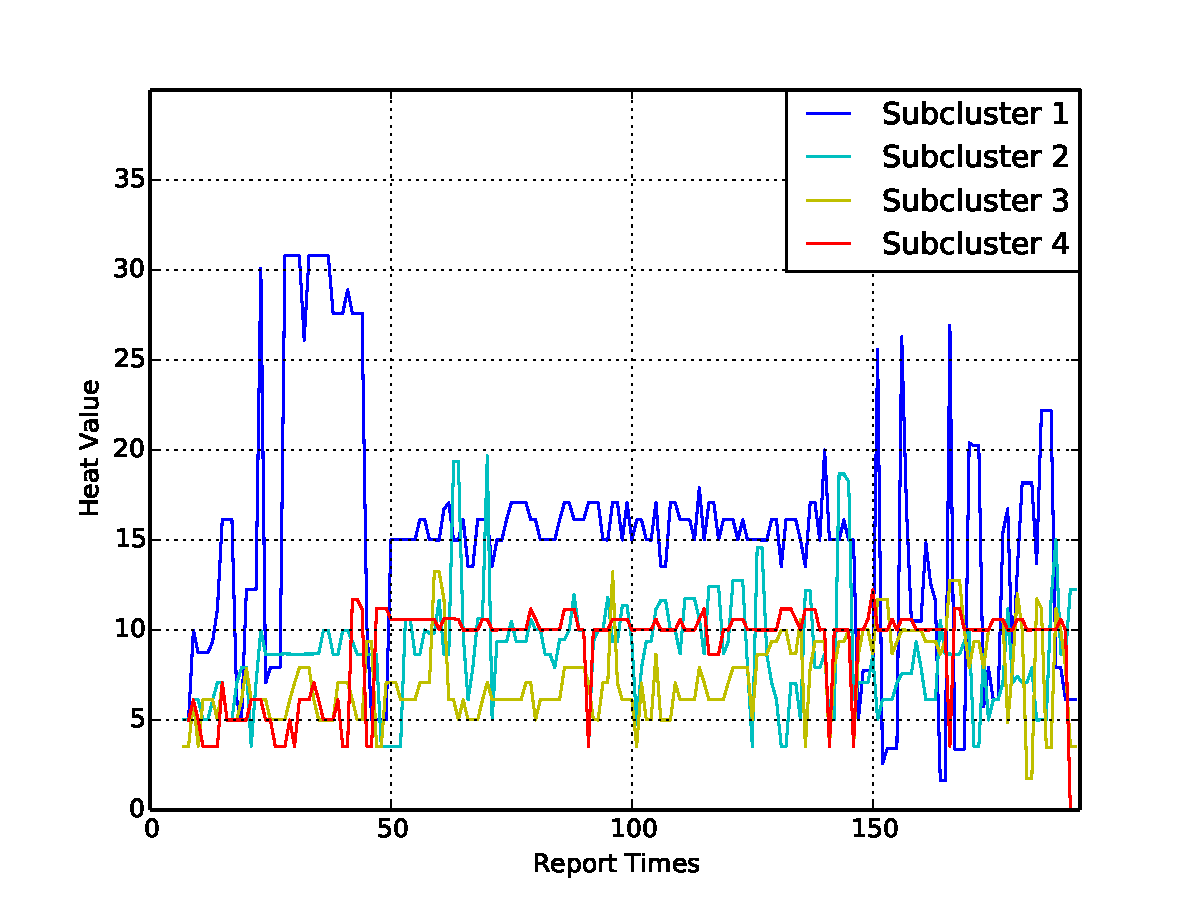
\includegraphics[width=9cm]{example/SingleMonitor.pdf}
    \bicaption[fig:singlemon]{关闭全局热均衡的DOBBS子集群热度值}{关闭全局热均衡的DOBBS子集群热度值}{Fig}{Heat Value of Subcluster without Global Heat Balancing}
\end{figure}

\begin{figure}[!htp]
    \centering
    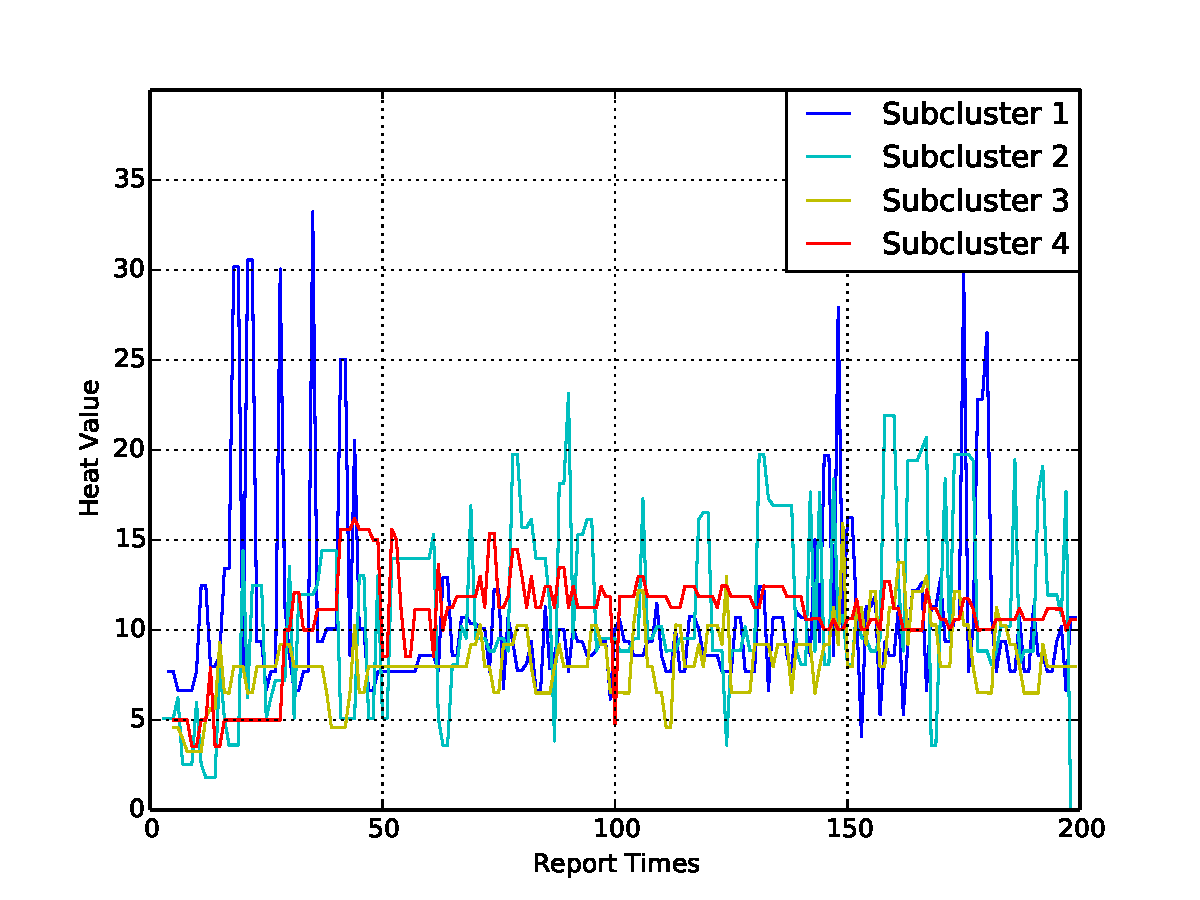
\includegraphics[width=9cm]{example/WithGHB.pdf}
    \bicaption[fig:withghb]{DOBBS的子集群热度值}{DOBBS的子集群热度值}{Fig}{Heat Value of Subcluster with Original DOBBS}
\end{figure}

考虑到全局热均衡的设计目标和实现目标,我们在验证全局热均衡有效性的时候将原始DOBBS(未做任何修改的DOBBS)与关闭了全局热均衡功能的DOBBS进行比较。我们知道,全局热均衡的根本目的是为了解决多个子集群后热度不均衡的情况,所以我们维持了
DOBBS的多子集群架构,但是只把全局热均衡功能关闭,来与原始DOBBS进行对比。图\ref{fig:singlemon}和图\ref{fig:withghb}分别表示关闭全局热均衡特性的子集群和原始DOBBS子集群的热度值随时间的变化。DOBBS的全局热均衡使得各个子集群的
热度值相对均衡,不会出现某个子集群热度值畸高的情况,DOBBS解决这个问题是通过将过热子集群的“热量”扩散到其他子集群来实现的。两个图中的纵坐标表示子集群的热度值,该热度值是在由公式\ref{eq:subheat}计算得出的,我们在每个Monitor加入了debug模块,
专门用来追踪热度值随时间的变化情况。横坐标为汇报时间,在这两个图中我们将汇报间隔平分成数个时间槽,并且每个时间槽都有相同的长度。为了测试全局热均衡的有效性,我们实现了一个没有Center节点的集群,在这个集群中的Monitor不会收集存储集群的IOPS也不会计算热度值,每个子集群都是独立的结构。
在测试的时候,我们设计了一个在VM上运行的独特的数据流。数据流的产生是通过修改一个叫做Filebench的基准测试工具实现的,我们将Filebench运行在Client的虚拟机上动态产生对虚拟机磁盘的访问请求。在本实验中,我们设置的热度阈值为30。

对于这两个实验,我们采取了一个相对极端的做法,我们将若干运行了Filebench的Client都接入在subcluster 1上,而其他子集群只是接入平稳运行虚拟机的Client。这个Filebench的数据流
实际上是模仿虚拟机的加载过程在开始会有一个大量访问增加的情况,之后会趋于平稳。

从图\ref{fig:singlemon}很清楚的看到,在20-45的时间槽内出现了一个连续的高峰,而其他子集群的热量则是处于很低的水平的。这是因为我们将所有数据流在加在subluster 1上。而在50-150的时间段内,
subcluster 1都一直处于热度值的高位,此时各个子集群之间的热度值标准差已经很大。从图\ref{fig:withghb}可以看出,采用同样的数据流,虽然在20-45的时间槽内出现过高峰,但是高峰并不平稳,而是立
刻降了下来,即使出现了新的高峰,也都可以快速地下降。观察其他子集群的热度值,可以显著得发现其他子集群的热度值相较于图\ref{fig:singlemon}有了显著提升,这就说明了全局热均衡把subcluster 1的热量分摊到了其他子集群。综上,我们可以证明全局热均衡可以消除一个子集群过热的情况。但是,我们需要注意的是,我们
定义热扩散是一个懒迁移过程,也就是说即使元数据被迁移之后,也需要等到局部热均衡来做后续的数据迁移工作。因此,我们从图\ref{fig:singlemon}和图\ref{fig:withghb}看到的subcluster 1的热度值
得到显著下降,大部分原因是元数据的迁移之后,Client开始向新的子集群发送数据信息导致的。而热扩散则是一个长期的过程,我们通过两张图并不能完全展现出来,因为它要配合局部热均衡才能实现,所以
时间会比较长。虽然没有在本文中呈现后续的实验结果,但是还是可以证明全局热均衡的有效的。

\begin{table}
    \centering
    \bicaption[tab:avgheat]{子集群的平均热度值}{子集群的平均热度值}{Table}{Average Heat Value of Subclusters}
    \begin{tabular}{@{}llr@{}} \toprule
       & Original DOBBS & without Heat Diffusion\\ \midrule
      subcluster 1 & 11.05 & 16.04 \\
      subcluster 2 & 10.69 & 9.0 \\
      subcluster 3 & 8.28 & 7.28 \\
      subcluster 4 & 10.73 & 8.75 \\
    \end{tabular}
\end{table}

我们不仅通过图的方式说明全局热均衡的有效性。表格\ref{tab:avgheat}所示,可以从数值上直观地看到各个子集群的平均热度值。明显的看到,subcluster 1在原生DOBBS下的热度值明显低于没有全局热均衡的DOBBS。
而其他子集群的热度值也明显有所增加,所有热度值的标准差明显减小。通过计算可以知道,原始DOBBS的四个子集群的平均热度标准差为1.28,而关闭全局热均衡的四个子集群的平均热度标准差为3.92。

尽管DOBBS消除了WHOBBS存在的性能问题并且全局热均衡又可以做到将过热的子集群的”热量“扩散到其他子集群上,可是在Client上运行的VM可能并不能获得比WHOBBS更好的性能提升。我们考虑到DOBBS的热扩散过程,
为了保证迁移过程中数据的一致性,防止热扩散的使能过程在传输元数据时和局部热均衡互相干扰,我们用try-lock机制来保护他们的相互影响。由try-lock机制我们可以知道,一旦对两个集群上锁,那么局部热均衡将
无法继续进行,同理在这个时间间隔内Client也无法向Monitor汇报对象的数据流信息。这样势必会影响Client上VM的运行。但是,这个影响其实也是微乎其微的,因为在我们大量试验下发现,热扩散的使能过程的耗时
基本上是小于200ms。所以,DOBBS相比于WHOBBS对Client上运行的VM并没有做到优化。

\section{软件定义存储验证}
上面的小节我们从系统性能的角度验证了与WHOBBS相比DOBBS Monitor的性能优势,以及DOBBS全局热均衡的有效性。本小节我们从功能的角度证明DOBBS是软件定义的存储系统。

在第\ref{chap:systemdesign}章的最后一节论证了DOBBS的局部热均衡和全局热均衡都是满足了软件定义系统的特性。首先对于局部热均衡,我们将子集群的控制面与存储面相分离,在实现过程中我们让每个子集群中的Monitor
收集和分析对象的数据流信息并发送迁移请求,同时它也会更新Client上的Object Table,这是控制面;我们通过修改Ceph和QEMU的源代码,让VM在IO请求之后先通过IO Controller查询到当前请求所对应的OSD ID,再交给
Ceph OSD Component进行后续的数据传输,由于IO Controller的存在,VM上的应用程序是不清楚对象具体在哪个OSD上的,这是存储面。表\ref{tab:mig}中的数据是我们从上一小节的原生DOBBS的子集群中获取到的,它表示了
各个子集群SSD和HDD间迁移对象的数量。可以看到每个子集群的从HDD到SSD的迁移数量都比SSD到HDD的数量多,这是因为我们在第\ref{chap:systemdesign}章的迁移策略是在一开始将所有对象通过热度排序后现将所有在对头的对象
移动到SSD上,所以这个时候会有大量的SSD到HDD的迁移,在SSD的数量满了之后就是根据迁移策略将对象在SSD和HDD间迁移。通过表格的数据可以证明,对象确实是在底层持续迁移的,而VM的应用程序仍然可以平稳正确的运行,因此
局部热均衡是软件定义的。

\begin{table}[!hpb]
    \centering
    \bicaption[tab:mig]{局部热均衡的迁移次数}{局部热均衡的迁移次数}{Table}{Migration Count of Local Heat Balancing}
    \begin{tabular}{@{}llr@{}} \toprule
      & SSD to HDD & HDD to SSD\\ \midrule
      subcluster 1 & 22 & 76 \\
      subcluster 2 & 11 & 57 \\
      subcluster 3 & 9 & 54 \\
      subcluster 4 & 9 & 55 \\
    \end{tabular}
\end{table}

对于全局热均衡的软件定义的验证实际我们已经在上一小节进行了验证,在全局热均衡的热扩散过程我们将subcluster 1的热量扩散到其他子集群的过程,实际就已经修改了子集群间的逻辑结构。在实验开始时,我们默认subcluster 1的OSD为1和2,subcluer 2的
OSD为3和4,以此类推。而实验结束之后,每个子集群的OSD编号都不再是系统初始化时候的编号。由此,我们也可以证明全局热均衡过程也是软件定义的。

\section{本章小结}
本章我们对DOBBS的系统设计和系统实现加以了实验上的论证。首先是对实现环境的搭建,我们配置了实验的硬件环境和软件环境。为了体现DOBBS消除了WHOBBS存在的性能问题,我们不仅部署了DOBBS在Monitor上,也配置了WHOBBS在Monitor上。本章第二节,我们引用了WHOBBS的论文结果论证了本文中的局部热均衡的高效性。其次,我们用WHOBBS的Monitor与DOBBS的Monitor做比,证明了DOBBS成功地消除WHOBBS的性能问题。之后,我们配置了一套不具有全局热均衡的DOBBS集群与原生DOBBS集群在相同数据流下作比较,实验结果可以明显的证明
DOBBS全局热均衡的有效性。第三节则论证了DOBBS的局部热均衡和全局热均衡过程都是软件定义的。
